\documentclass[12pt]{article}

\title{\vspace{-3em}PHYS 167b HW 7}
\author{Michael Cardiff}
\date{\today}

%% science symbols
\usepackage{amsmath}
\usepackage{amssymb}
\usepackage{amsthm}
\usepackage{bm}
\usepackage{cancel}
\usepackage{physics}
\usepackage{siunitx}
\usepackage{slashed}

%% general pretty stuff
\usepackage{caption}
\usepackage{float}
\usepackage{graphicx}
\usepackage{url}
\usepackage{enumitem}
\usepackage{hyperref}
\usepackage{tikz}
\usepackage{tikz-feynhand}
\usepackage[margin=1in]{geometry}

% setup options
\captionsetup{labelfont=bf}
\graphicspath{ {./figs/} }

% macros
\renewcommand{\L}{\mathcal{L}}
\renewcommand{\H}{\mathcal{H}}
\renewcommand{\l}{\ell}
\newcommand{\M}{\mathcal{M}}
\newcommand{\mcV}{\mathcal{V}}
\newcommand{\D}{\partial}
\newcommand{\veps}{\varepsilon}
\newcommand{\circled}[1]{\tikz[baseline=(char.base)]{
    \node[shape=circle,draw,inner sep=2pt](char){#1};}}

% mdframed environments
\usepackage[framemethod=TikZ]{mdframed}
\mdfsetup{skipabove=\topskip,skipbelow=\topskip}
\mdfdefinestyle{defstyle}{%
  linewidth=1pt,
  frametitlerule=true,
  frametitlebackgroundcolor=gray!40,
  backgroundcolor=gray!20,
  innertopmargin=\topskip
}

\mdtheorem[style=defstyle]{definition}{Definition}
\mdtheorem[style=defstyle]{theorem}{Theorem}
\mdtheorem[style=defstyle]{problem}{Problem}

\newenvironment{thebook}
{\begin{mdframed}[style=defstyle,frametitle={From the Book}]}{\end{mdframed}}

\begin{document}
\maketitle
\section{Thomson, Problem 15.1}
\begin{problem}
  Draw all possible lowest-order Feynman diagrams for the processes:
  \begin{align*}
    e^+e^-\to\mu^+\mu^-,\enspace
    e^+e^-\to\nu_\mu\overline{\nu}_\mu,\enspace
    \nu_\mu e^-\to\nu_\mu e^-,\enspace\,\text{and}\enspace\,
    \overline{\nu}_e e^-\to\overline{\nu}_e e^-
  \end{align*}
\end{problem}
\begin{itemize}
\item $e^+e^-\to\mu^+\mu^-$
  \begin{figure}[H]
    \centering
    \begin{tikzpicture}[scale=1.5]
      \node at (0.0,0) {$e$};
      \node at (1.9,0) {$e$};
      \begin{feynhand}
        % vertices
        \vertex (p11) at (-1,1) {$e^-$};
        \vertex (p12) at (-1,-1) {$e^+$};
        \vertex (p21) at (3,1) {$\mu^-$};
        \vertex (p22) at (3,-1) {$\mu^+$};
        \vertex (a) at (0.3,0);
        \vertex (b) at (1.7,0);
        % particles
        \propag [fer] (p11) to (a);
        \propag [antfer] (p12) to (a);
        \propag [fer] (b) to (p21);
        \propag [antfer] (b) to (p22);
        % loop
        \propag [bos] (a) to [edge label=$\gamma$] (b);
      \end{feynhand}
    \end{tikzpicture}
    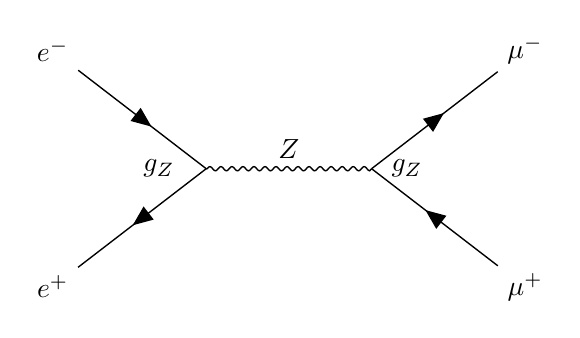
\begin{tikzpicture}[scale=1.5]
      \node at (-0.1,0) {$g_Z$};
      \node at (2.0,0) {$g_Z$};
      \begin{feynhand}
        % vertices
        \vertex (p11) at (-1,1) {$e^-$};
        \vertex (p12) at (-1,-1) {$e^+$};
        \vertex (p21) at (3,1) {$\mu^-$};
        \vertex (p22) at (3,-1) {$\mu^+$};
        \vertex (a) at (0.3,0);
        \vertex (b) at (1.7,0);
        % particles
        \propag [fer] (p11) to (a);
        \propag [antfer] (p12) to (a);
        \propag [fer] (b) to (p21);
        \propag [antfer] (b) to (p22);
        % loop
        \propag [bos] (a) to [edge label=$Z$] (b);
      \end{feynhand}
    \end{tikzpicture}
    \caption{Diagrams for $e^+e^-\to\mu^+\mu^-$}\label{fig:p1a}
  \end{figure}
\item $e^+e^-\to\nu_\mu\overline{\nu}_\mu$
  \begin{figure}[H]
    \centering
    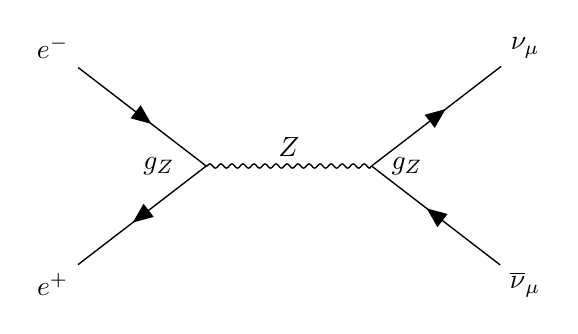
\begin{tikzpicture}[scale=1.5]
      \node at (-0.1,0) {$g_Z$};
      \node at ( 2.0,0) {$g_Z$};
      \begin{feynhand}
        % vertices
        \vertex (p11) at (-1,1) {$e^-$};
        \vertex (p12) at (-1,-1) {$e^+$};
        \vertex (p21) at (3,1) {$\nu_\mu$};
        \vertex (p22) at (3,-1) {$\overline{\nu}_\mu$};
        \vertex (a) at (0.3,0);
        \vertex (b) at (1.7,0);
        % particles
        \propag [fer] (p11) to (a);
        \propag [antfer] (p12) to (a);
        \propag [fer] (b) to (p21);
        \propag [antfer] (b) to (p22);
        % loop
        \propag [bos] (a) to [edge label=$Z$] (b);
      \end{feynhand}
    \end{tikzpicture}
    \caption{Diagram for $e^+e^-\to\nu_\mu\overline{\nu}_\mu$}\label{fig:p1b}
  \end{figure}
\item $\nu_\mu e^-\to\nu_\mu e^-$
  \begin{figure}[H]
    \centering
    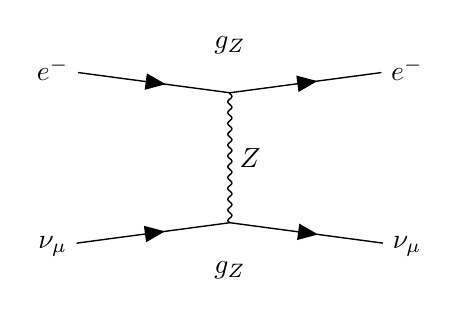
\begin{tikzpicture}[scale=1.5]
      \node at (0,-0.2) {$g_Z$};
      \node at (0,1.7) {$g_Z$};
      \begin{feynhand}
        % vertices
        \vertex (p11) at (1.5,0) {$\nu_\mu$};
        \vertex (p21) at (1.5,1.5) {$e^-$};
        \vertex (p12) at (-1.5,0) {$\nu_\mu$};
        \vertex (p22) at (-1.5,1.5) {$e^-$};
        \vertex (a) at (0,0.2); \vertex (b) at (0,1.3);
        % particles
        \propag [fer] (p22) to (b);
        \propag [fer] (p12) to (a);
        \propag [fer] (b) to (p21);
        \propag [fer] (a) to (p11);
        % exchange
        \propag [bos] (b) to [edge label=$Z$] (a);
      \end{feynhand}
    \end{tikzpicture}
    \caption{Diagram for $\nu_\mu e^-\to\nu_\mu e^-$}\label{fig:p1c}
  \end{figure}
\item $\overline{\nu}_e e^-\to\overline{\nu}_e e^-$
  \begin{figure}[H]
    \centering
    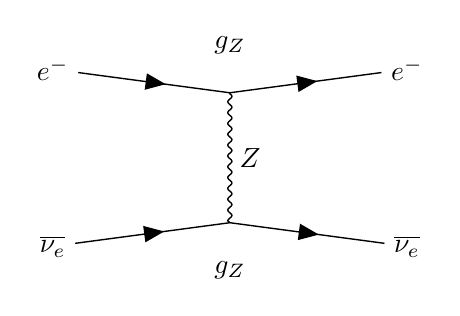
\begin{tikzpicture}[scale=1.5]
      \node at (0,-0.2) {$g_Z$};
      \node at (0,1.7) {$g_Z$};
      \begin{feynhand}
        % vertices
        \vertex (p11) at (1.5,0) {$\overline{\nu_e}$};
        \vertex (p21) at (1.5,1.5) {$e^-$};
        \vertex (p12) at (-1.5,0) {$\overline{\nu_e}$};
        \vertex (p22) at (-1.5,1.5) {$e^-$};
        \vertex (a) at (0,0.2); \vertex (b) at (0,1.3);
        % particles
        \propag [fer] (p22) to (b);
        \propag [fer] (p12) to (a);
        \propag [fer] (b) to (p21);
        \propag [fer] (a) to (p11);
        % exchange
        \propag [bos] (b) to [edge label=$Z$] (a);
      \end{feynhand}
    \end{tikzpicture}
        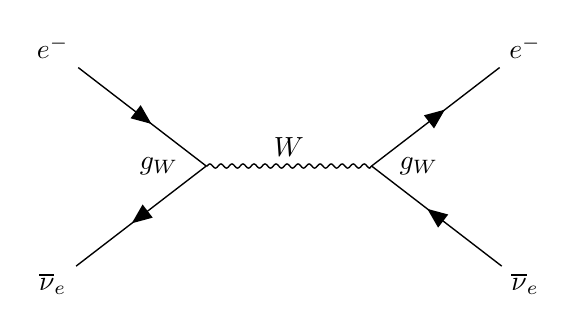
\begin{tikzpicture}[scale=1.5]
      \node at (-0.1,0) {$g_W$};
      \node at (2.1,0) {$g_W$};
      \begin{feynhand}
        % vertices
        \vertex (p11) at (-1,1) {$e^-$};
        \vertex (p12) at (-1,-1) {$\overline{\nu}_e$};
        \vertex (p21) at (3,1) {$e^-$};
        \vertex (p22) at (3,-1) {$\overline{\nu}_e$};
        \vertex (a) at (0.3,0);
        \vertex (b) at (1.7,0);
        % particles
        \propag [fer] (p11) to (a);
        \propag [antfer] (p12) to (a);
        \propag [fer] (b) to (p21);
        \propag [antfer] (b) to (p22);
        % loop
        \propag [bos] (a) to [edge label=$W$] (b);
      \end{feynhand}
    \end{tikzpicture}
    \caption{Diagrams for $\overline{\nu}_e e^-\to\overline{\nu}_e e^-$}\label{fig:p1d}
  \end{figure}
\end{itemize}
\newpage
\section{Thomson, Problem 15.3}
\begin{problem}
  Starting from the matrix element, work through the calculation of the $Z\to f\overline{f}$ partial decay rate, expressing the answer in terms of the vector and axial-vector couplings of $Z$. Taking $\sin^2\theta_W=0.2315$, show that
  \begin{align*}
    R_\mu=\frac{\Gamma(Z\to\mu^+\mu^-)}{\Gamma(Z\to\text{hadrons})}
    \approx\frac1{20}
  \end{align*}
\end{problem}
The $Z\to f\overline{f}$ decay is given by the following diagram:
\begin{figure}[H]
  \centering
  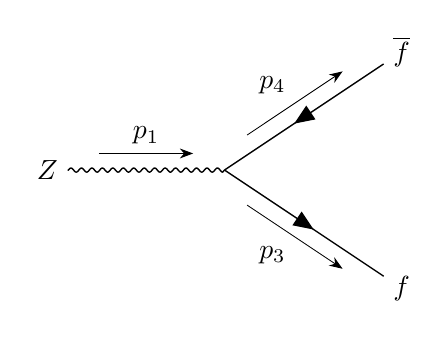
\begin{tikzpicture}[scale=1.5]
    \begin{feynhand}
      \vertex (zl) at (-1.5,0) {$Z$};
      \vertex (zr) at (0,0);
      \vertex (fb) at (1.5,1) {$\overline{f}$};
      \vertex (f) at (1.5,-1) {$f$};
      \propag [bos, mom=\(p_1\)] (zl) to (zr);
      \propag [fer, mom'=\(p_3\)] (zr) to (f);
      \propag [antfer, mom=\(p_4\)] (zr) to (fb);
    \end{feynhand}
  \end{tikzpicture}
  \caption{Diagram for $Z\to f\overline{f}$}\label{fig:p2}
\end{figure}
Where the matrix element is given by:
\begin{align*}
  \M_{fi}=\veps_\mu^\lambda(p_1)\overline{u}(p_3)
  g_Z\gamma^\mu\qty[c_L\frac12(1-\gamma^5)+c_R\frac12(1+\gamma^5)]
  v(p_4)
\end{align*}
Where $\mu$ is a spacetime index and $\lambda$ is a polarization index. Since this includes the chiral projection operators, so the only chiral combinations that will work are with a LH particle and RH antiparticle, where only the $c_L$ term contributes, as well as a RH particle and LH antiparticle, where only the $c_R$ term contributes. Taking the ultra-relativistic limit, the helicity states are:
\begin{align*}
  \M_{LR}&=g_Z c_L\veps_\mu^\lambda(p_1)\overline{u_\downarrow}(p_3)
  \gamma^\mu v_\uparrow(p_4)\\
  \M_{RL}&=g_Z c_L\veps_\mu^\lambda(p_1)\overline{u_\uparrow}(p_3)
  \gamma^\mu v_\downarrow(p_4)
\end{align*}
We have calculated these several times before, and know that the fermion currents are given by:
\begin{align*}
  j^\mu_{LR}&=m_Z(0,-\cos\theta,-i,\sin\theta)\\
  j^\mu_{RL}&=m_Z(0,-\cos\theta,+i,\sin\theta)
\end{align*}
We can take the frame to be the rest frame of the $Z$, and choose its polarization, since it would not change the dynamics if it was polarized differently:
\begin{align*}
  \veps^\lambda_\mu=\veps^0_\mu=(0,0,0,1)
\end{align*}
As given in the appendix, so we only take out the $3$ index of the current, such that:
\begin{align*}
  \M_{LR}&=-g_Z c_L j^3_{LR}=-g_Z c_L m_Z\sin\theta\\
  \M_{LR}&=-g_Z c_R j^3_{RL}=-g_Z c_R  m_Z\sin\theta
\end{align*}
The total decay rate is then given by the square of this:
\begin{align*}
  \abs{\M}^2=\abs{\M_{LR}}^2+\abs{\M_{RL}}^2=g_Z^2m_Z^2(c_L^2+c_R^2)\sin^2\theta
\end{align*}
Plugging this into the total decay rate formula:
\begin{align*}
  \Gamma(Z\to f\overline{f})=\frac{p^*}{32\pi^2m_Z^2}\int\abs{\M}^2\dd{\Omega}
\end{align*}
The momentum $p^*$ should just be half the $Z$ mass, since we are already ignoring the fermion masses by taking the ultra-relativistic limit, hence we get:
\begin{align*}
  \Gamma(Z\to f\overline{f})&=\frac1{64\pi^2m_Z}\int\abs{\M}^2\dd{\Omega}
  =\frac{g_Z^2m_Z}{64\pi^2}(c_L^2+c_R^2)\int\sin^2\theta\dd{\Omega}\\
  &=\frac{g_Z^2m_Z}{32\pi}(c_L^2+c_R^2)
  \int_{-1}^1\sin^2\theta\dd{(\cos\theta)}\\
  &=\frac{g_Z^2m_Z}{32\pi}(c_L^2+c_R^2)
  \int_{-1}^1(1-z^2)\dd{z}\\
  &=\frac{g_Z^2m_Z}{24\pi}(c_L^2+c_R^2)
\end{align*}
The $V$ and $A$ constants are a bit easier to work with, so we get that:
\begin{align*}
  \Gamma(Z\to f\overline{f})=\frac{g_Z^2m_Z}{48\pi}(c_V^2+c_A^2)
\end{align*}
We then have the partial widths given in the ratio $R_\mu$:
\begin{align*}
  \Gamma(Z\to\text{hadrons})=
  3\Gamma(Z\to u\overline{u})+3\Gamma(Z\to d\overline{d})\\+
  3\Gamma(Z\to c\overline{c})+3\Gamma(Z\to s\overline{s})\\+
  3\Gamma(Z\to b\overline{b})
\end{align*}
Where we have accounted for the colors and the fact that $Z$ cannot decay to top, but for several of these they are the same due to the similar $c_V/c_A$:
\begin{align*}
  \Gamma(Z\to\text{hadrons})=
  9\Gamma(Z\to d\overline{d})+6\Gamma(Z\to u\overline{u})
\end{align*}
Then the numerator is just the partial width to a $\mu$ pair, we can then identify the constants for each of these:
\begin{align*}
  {(c_V^{(\mu)})}^2+{(c_A^{(\mu)})}^2=0.2516,\quad
  {(c_V^{(d)})}^2+{(c_A^{(d)})}^2=0.3725,\quad
  {(c_V^{(u)})}^2+{(c_A^{(u)})}^2=0.2861
\end{align*}
Plugging these in:
\begin{equation}
  \label{eq:p2}
  \boxed{R_\mu\approx0.49\approx\frac1{20}}
\end{equation}
Which is the desired result
\newpage
\section{Thomson, Problem 16.1}
\begin{problem}
  After correcting for QED effects, including initial-state radiation, the measured $e^+e^-\to\mu^+\mu^-$ and $e^+e^-\to\text{hadrons}$ cross sections at the peak of the $Z$ resonance give:
  \begin{align*}
    \sigma^0(e^+e^-\to Z\to \mu^+\mu^-)=1.9993\text{ nb}\,\,\text{and}\,\,
    \sigma^0(e^+e^-\to Z\to\text{hadrons})=41.476\text{ nb}.
  \end{align*}
  \begin{enumerate}[label = (\alph*)]
  \item Assuming lepton universality, determine $\Gamma_{\l\l}$ and $\Gamma_{\text{hadrons}}$.
  \item Hence, using the value of $\Gamma_Z=2.4952\pm0.0023\text{ GeV}$ and the theoretical of $\Gamma_{\nu\nu}$ given by Equation (15.41), obtain an estimate of the number of light neutrino flavors.
  \end{enumerate}
\end{problem}
The peak of the cross section $\sigma^0_{ff}$ is given by:
\begin{align*}
  \sigma^0_{ff}=\frac{12\pi}{m_Z^2}\frac{\Gamma_{ee}\Gamma_{ff}}{\Gamma_Z^2}
\end{align*}
Rearrange to solve for the product term:
\begin{align*}
  \Gamma_{ee}\Gamma_{ff}=\frac{\sigma_{ff}^0\Gamma_Z^2m_Z^2}{12\pi}
\end{align*}
Lepton universality, in the case where $ff=\mu\mu$, we can replace $\Gamma_{ee}$ with $\Gamma_{\l\l}$ to find that:
\begin{align*}
  \Gamma^2_{\l\l}=\frac{\sigma^0_{\mu\mu}\Gamma_Z^2m_Z^2}{12\pi}
\end{align*}
The natural units measurement for the cross section peak is given by:
\begin{align*}
  \sigma^0_{\mu\mu}=\SI{1.9993e-37}{m^2}(\hbar c)^{-2}=\SI{5.152e-6}{GeV^{-2}}
\end{align*}
Using the $Z$ mass as $\SI{91.2}{GeV}$ we then find that:
\begin{align*}
  \Gamma_{\l\l}^2\approx\num{1.137e-3}\Gamma_{Z}^2
\end{align*}
Giving $\Gamma_{\l\l}$ as:
\begin{equation}
  \label{eq:p3a}
  \boxed{\Gamma_{\l\l}=0.0337\Gamma_Z}
\end{equation}
Using this for $\Gamma_{\text{hadrons}}$:
\begin{align*}
  \Gamma_{\l\l}\Gamma_{\text{hadrons}}&=
  \frac{\sigma^0_{\text{hadrons}}\Gamma_Z^2m_Z^2}{12\pi}\\
  &\approx0.024\Gamma_Z^2
\end{align*}
Subbing in $\Gamma_{\l\l}$ from before leads to:
\begin{equation}
  \label{eq:p3b}
  \boxed{\Gamma_{\text{hadrons}}\approx0.6994\Gamma_Z}
\end{equation}
For the next part, we can write the total $Z$ width as a sum of partial widths, leaving the number of (light) neutrino flavors as variable:
\begin{align*}
  \Gamma_Z=\Gamma_{\text{hadrons}}+3\Gamma_{\l\l}+N_\nu\Gamma_{\nu\nu}
\end{align*}
We were given a value of $\Gamma_Z$, so we can solve for $N_\nu\Gamma_{\nu\nu}$:
\begin{align*}
  N_\nu\Gamma_{\nu\nu}=(1-3(0.00337)-(0.6994))\Gamma_Z\approx\SI{0.497}{GeV}
\end{align*}
The neutrino width of the $Z$ was earlier calculated to be $\SI{0.167}{GeV}$, plugging this in gives an estimate of $N_\nu$:
\begin{equation}
  \label{eq:p3c}
  \boxed{N_\nu=\frac{\Gamma_Z-\Gamma_{\text{hadrons}}-3\Gamma_{\l\l}}{\Gamma_{\nu\nu}}\approx2.98}
\end{equation}
Which, given the uncertainties of the various quantities we have used in this problem, is consistent with what we have observed.
\newpage
\section{Thomson, Problem 16.2}
\begin{problem}
  Show that $e^+e^-\to Z\to \mu^+\mu^-$ differential cross secttion can be written as:
  \begin{align*}
    \dv{\sigma}{\Omega}\propto(1+\cos^2\theta)+\frac83A_{FB}\cos\theta
  \end{align*}
\end{problem}
The book gives the following form for the $Z$
\begin{align*}
  \dv{\sigma}{\Omega}\propto a(1+\cos^2\theta)+2b\cos\theta
\end{align*}
Where $a$ and $b$ are given in terms of the $c_{L/R}$ of the $\mu/e$.

We want to write this in terms of the forward backwards asymmetry factor, we need to calculate the number of events in the forward and backward regions. In general, the ``forward'' region is defined by $0<\cos\theta<1$, and the ``backwards'' region is $-1<\cos\theta<0$, so we find two things:
\begin{align*}
  A_{FB}&=\frac{N_F-N_B}{N_F+N_B}\\
  N_{F/B}&=\int_{F/B}\dv{\sigma}{\Omega}\dd{\Omega}
\end{align*}
We can also write the cross section including a normalization constant, call it $N$, such that $N$ is defined to satisfy:
\begin{align*}
  \dv{\sigma}{\Omega}=N\qty[a(1+\cos^2\theta)+2b\cos\theta]
\end{align*}
We can then perform the integrals, noting $z=\cos\theta$:
\begin{align*}
  N_F&=2\pi N\int_0^1\qty[a(1+z^2)+2bz]\dd{z}=2N\pi\qty[\frac43a+b]\\
  N_B&=2\pi N\int_{-1}^0\qty[a(1+z^2)+2bz]\dd{z}=2N\pi\qty[\frac43a-b]
\end{align*}
Plugging these values into the formula for $A_{FB}$ gives:
\begin{align*}
  A_{FB}=\frac{3b}{4a}
\end{align*}
Which means in our formula, we can sub $b$ as:
\begin{align*}
  b=\frac{4a}{3}A_{FB}
\end{align*}
Meaning we can remove $a$ from the proportionality, leaving us with:
\begin{equation}
  \label{eq:p4}
  \boxed{\dv{\sigma}{\Omega}\propto(1+\cos^2\theta)+\frac83A_{FB}\cos\theta}
\end{equation}

\newpage
\section{Thomson, Problem 17.2}
\begin{problem}
  The Lagrangian for the Dirac Equation is
  \begin{align*}
    \L=i\overline{\psi}\gamma_\mu\D^\mu\phi-m\overline{\psi}\psi
  \end{align*}
  Treating the eight fields $\psi_i$ and $\overline{\psi}_i$ as independent, show that the Euler-Lagrange equation for the component $\psi_i$ leads to
  \begin{align*}
    i\D_\mu\overline{\psi}\gamma^\mu+m\overline{\psi}=0
  \end{align*}
\end{problem}
The derivatives we need for the Euler-Lagrange equations are:
\begin{align*}
  \pdv{\L}{(\D_\mu\psi)}&=i\overline{\psi}\gamma^\mu
  \pdv{(\D_\mu\psi)}{(\D_\mu\psi)}=i\overline{\psi}\gamma^\mu\\
  \D_\mu\qty(\pdv{\L}{(\D_\mu\psi)})&=\D_\mu(i\overline{\psi}\gamma^\mu)\\
  \pdv{\L}{\psi}&=-m\overline{\psi}\pdv{\psi}{\psi}=-m\overline{\psi}
\end{align*}
Hence the Euler Lagrange equations give the adjoint Dirac equation:
\begin{equation}
  \label{eq:p5}
  \D_\mu\qty(\pdv{\L}{(\D_\mu\psi)})-\pdv{\L}{\psi}=0\implies
  \boxed{i(\D_\mu\overline{\psi}\gamma^\mu)+m\overline{\psi}=0}
\end{equation}
\newpage
\section{Thomson, Problem 16.4}
\begin{problem}
  The $e^+e^-$ Stanford Linear Collider (SLC), operated at $\sqrt{s}=m_Z$ with left- and right-handed longitudinally polarized beams. This enabled the $e^+e^-\to Z\to f\overline{f}$ cross section to be measured separately for left-handed and right-handed electrons.

  Assuming that the electron beam is 100\% polarized and that the positron beam is unpolarized, show that the left-right asummetry $A_{LR}$ is given by:
  \begin{align*}
    A_{LR}=\frac{\sigma_L-\sigma_R}{\sigma_L+\sigma_R}
    =\frac{(c^e_L)^2-(c^e_R)^2}{(c^e_L)^2+(c^e_R)^2}=\mathcal{A}_e
  \end{align*}
  Where $\sigma_L$ and $\sigma_R$ are respectively the measured cross sections at the $Z$ resonance for $LH$ and $RH$ electron beams.
\end{problem}
In class we calculated the various matrix elements for the proper helicity combinations, given in the book starting  wtih eq. (16.9).

First we need to calculate the positron helicity averaged matrix elements:
\begin{align*}
  \ev{\abs{\M_L}^2}&=\frac12\qty[\abs{\M_{LR\to RL}}^2+\abs{\M_{LR\to LR}}^2]\\
  &=\frac12\abs{P_Z(s)}^2g_Z^4s^2(c_L^e)^2
  \qty[(c_R^\mu)^2(1-\cos\theta)^2+(c_L^\mu)^2(1+\cos\theta)^2]\\
  \ev{\abs{\M_R}^2}&=\frac12\qty[\abs{\M_{RL\to RL}}^2+\abs{\M_{RL\to LR}}^2]\\
  &=\frac12\abs{P_Z(s)}^2g_Z^4s^2(c_R^e)^2
  \qty[(c_R^\mu)^2(1+\cos\theta)^2+(c_L^\mu)^2(1-\cos\theta)^2]
\end{align*}
Computing the $LR$ cross sections only requires doing two integrals, with $z=\cos\theta$:
\begin{align*}
  \int_{-1}^1(1+z)^2\dd{z}=\frac83=\int_{-1}^1(1-z)^2\dd{z}
\end{align*}
Now the $A_{LR}$ becomes:
\begin{align*}
  A_{LR}&=\frac{\sigma_L-\sigma_R}{\sigma_L+\sigma_R}=
  \frac{(c^e_L)^2\frac83\qty[(c^\mu_R)^2+(c^\mu_L)^2]+
    (c^e_R)^2\frac83\qty[(c^\mu_R)^2+(c^\mu_L)^2]}{
    (c^e_L)^2\frac83\qty[(c^\mu_R)^2+(c^\mu_L)^2]-
    (c^e_R)^2\frac83\qty[(c^\mu_R)^2+(c^\mu_L)^2]
  }\\
  &=\frac{(c^e_L)^2\qty[(c^\mu_R)^2+(c^\mu_L)^2]+
    (c^e_R)^2\qty[(c^\mu_R)^2+(c^\mu_L)^2]}{
    (c^e_L)^2\qty[(c^\mu_R)^2+(c^\mu_L)^2]-
    (c^e_R)^2\qty[(c^\mu_R)^2+(c^\mu_L)^2]}\\
  &=\frac{(c^e_L)^2+(c^e_R)^2}{(c^e_L)^2-(c^e_R)^2}
\end{align*}
Which is precisely $\mathcal{A}_e$, hence:
\begin{equation}
  \label{eq:p6}
  \boxed{A_{LR}=\mathcal{A}_e}
\end{equation}
\end{document}